%\RequirePackage{plautopatch} % パッチを自動的に適用してくれる

% 仕様 ----------------------------------------------------------------------------------------------------------------

\documentclass[b5paper,11pt,dvipdfmx]{jsarticle}
\usepackage{amsmath,amssymb,amsthm,amsfonts}
\usepackage{hyperref}
\usepackage{mathtools}
\usepackage{graphicx}
\usepackage{url}
\usepackage{calligra}
\usepackage{physics}
\usepackage{tikz}
\usepackage{tcolorbox}
\usepackage{mathcomp}
\usepackage{textcomp}
\usepackage{pxjahyper}

\numberwithin{equation}{section}
\theoremstyle{definition}
\newtheorem{thm}{定理}[section]
\newtheorem{lem}[thm]{補題}
\newtheorem{prop}[thm]{命題}
\newtheorem{cor}[thm]{系}
\newtheorem{ass}[thm]{仮定}
\newtheorem{conj}[thm]{予想}
\newtheorem{dfn}[thm]{定義}
\newtheorem{rem}[thm]{注}


% 追加するパッケージたち ----------------------------------------------------------------------------------------------------------------

\usepackage{mathrsfs} % 花文字をいれる
\usepackage{bm,ascmac,latexsym,color}
\usepackage{varwidth}
\usepackage{pxrubrica}
\usepackage{titlesec}
\usepackage{tocloft}

\usetikzlibrary{calc}
\tcbuselibrary{raster,breakable,theorems,skins}


% プリアンブルおわり ==============================================================

\begin{document}

\title{ホログラフィック超伝導の進展から}
\author{川合玲央}
\date{}

\maketitle

%\tableofcontents

\begin{abstract}
    皆さんはホログラフィー原理,もしくはAdS/CFT対応という言葉を聞いたことがあるでしょうか?
    本記事ではホログラフィー原理による超伝導現象の解析の試みと,特にその近年の進展について紹介します.
    ホログラフィー原理とは重力理論とゲージ理論が等価であるという主張であり,
    量子重力理論の構築への足がけとして期待されている枠組みです.
    そんな熱い期待\footnote{筆者の主観です.}がかけられているホログラフィー原理は,実はその端緒を弦理論にもちます.
    にもかかわらず弦理論がよく言われる検証不可能性
\footnote{弦理論の典型的なエネルギースケールは$10^{19}$GeV程度であり,
現在稼働している加速器のエネルギースケールは$10^4$GeV程度です.
かなりの差がありますね.この事実をもってして弦理論は現実的な観点から検証不可能であると言われたりすることがあります.
ただ高エネルギースケールの弦理論から示唆される結果は,弦理論それ自体の検証ができなくとも
我々がよく知っている現実的なスケールの物理も含んでいると期待しているわけですから,
それら低エネルギー有効理論に対する制限を与えるなど多くの場面で有用です.
ホログラフィー原理もその一種だと思っています.
またstring phenomenologyという分野もあると聞きますが,筆者はその有用性と詳細を知らないので言及しません.}
にとらわれず,実際に現実の観測量と結びつける研究が多数行われています.
よく挙げられる例としてはクォーク・グルーオン・プラズマ\cite{Policastro01,Kovtun04}
や超伝導\cite{Hartnoll08a,Hartnoll08b}があります.
今回は超伝導(正確には超伝導っぽいもの)をホログラフィー原理を用いて解析
\end{abstract}


\section{導入}


\subsection{ホログラフィー原理}
ホログラフィー原理を知っているか?
ここがすごい!ホログラフィー原理
AdS/CFT対応ともよばれ,
$d + 2$次元の重力理論と$d + 1$次元のゲージ理論が等価になるという主張.
1997年にMaldacenaにより最初の例が示された\cite{Maldacena97}.

\begin{figure}[t]
    \centering
    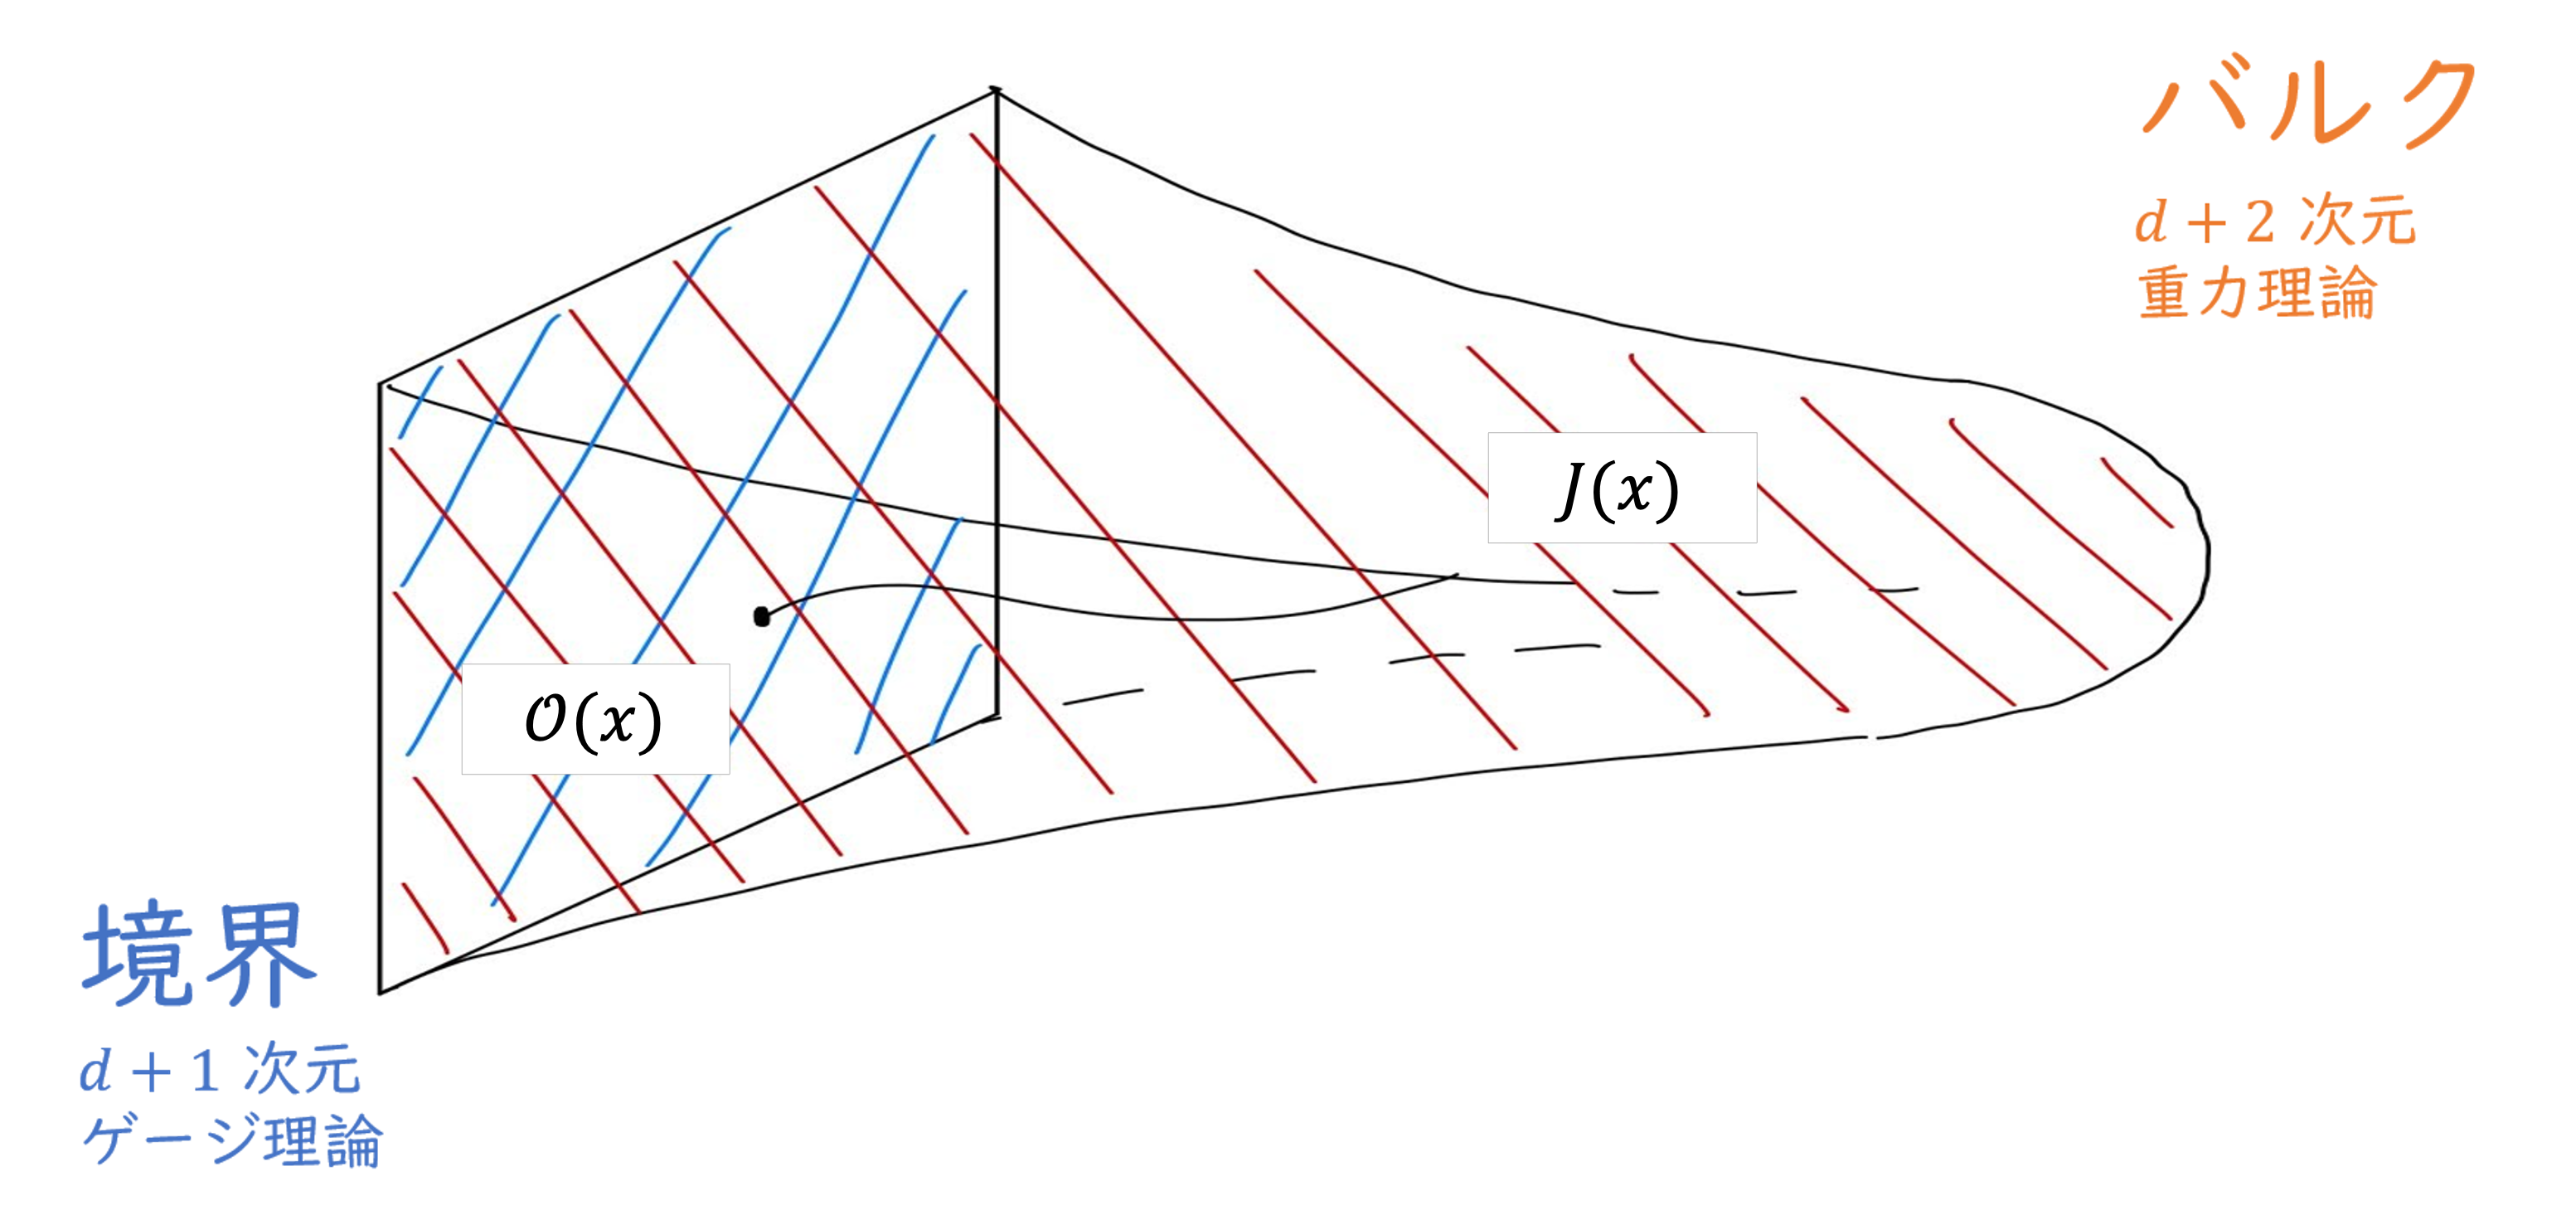
\includegraphics[width=0.9\textwidth]{holography.png}
    \caption{ホログラフィー原理の概念図}
    \label{fig:holography}
\end{figure}


GKP--Witten関係式
バルク中の場$\mathcal{J}(x)$が
境界上の物理量$\mathcal{O}(x)$のソースとなる
\cite{Gubser98,Witten98}


\subsubsection{QGP}
BNLのレポート
弦理論が役にたつ
実験結果$\frac{\eta}{s} \approx 0.1$,
ホログラフィーによる計算$\frac{\eta}{s} = \frac{1 \hbar}{4 \pi k_B} \approx 0.08$.

実験レポート
\cite{PHENIX06}

引用されている粘性の予言
\cite{Kovtun04}

QGPにおける「成功」があった
他の例にも応用したい
とりあえず同じような強結合の場に応用してみる
物性においてはそのような強相関系

中村真の仕事で、時間依存する重力時空と流体力学の関係、および時空の正則性と
流体の輸送係数を論じた代表的な論文は
S. Kinoshita, S. Mukohyama, S. Nakamura and K. y. Oda, “Consistent Anti-de
Sitter-Space/Conformal-Field-Theory Dual for a Time-Dependent Finite Tem-
perature System,” Phys. Rev. Lett. 102 (2009) 031601 [arXiv:0901.4834 [hep-
th]];
S. Kinoshita, S. Mukohyama, S. Nakamura and K. y. Oda, “A Holographic
Dual of Bjorken Flow,” Prog. Theor. Phys. 121 (2009) 121 [arXiv:0807.3797
[hep-th]].
なお、これら一連の仕事の発端となった研究は、
R. A. Janik and R. B. Peschanski, “Asymptotic perfect fluid dynamics as
a consequence of AdS/CFT,” Phys. Rev. D 73, 045013 (2006) [arXiv:hep-
th/0512162].




解析手段としてのホログラフィー原理
→ RHICにおける成功
• その他の強結合ゲージ場への応用
→ 高温超伝導に対する期待
• ホログラフィック超伝導にあった問題点の解決
→ 境界上の電磁場にダイナミクスを導入



ホログラフィック超伝導というのがあるよ

強結合、つまり高温超伝導を解決できるかもしれないよ

ホログラフィーっていうのは場の理論の問題を重力を使って簡単に解くことができる手法だよ

従来のホログラフィック超伝導はゲージ場がダイナミカルじゃないから問題だよ
(例えばMeissner効果が起きないよ???)

最近提唱されたモデルではMeissner効果が起きるなど従来の問題を解決したよ





















\section{ホログラフィック超伝導}

\subsection{高温超伝導}
\begin{figure}[t]
    \centering
    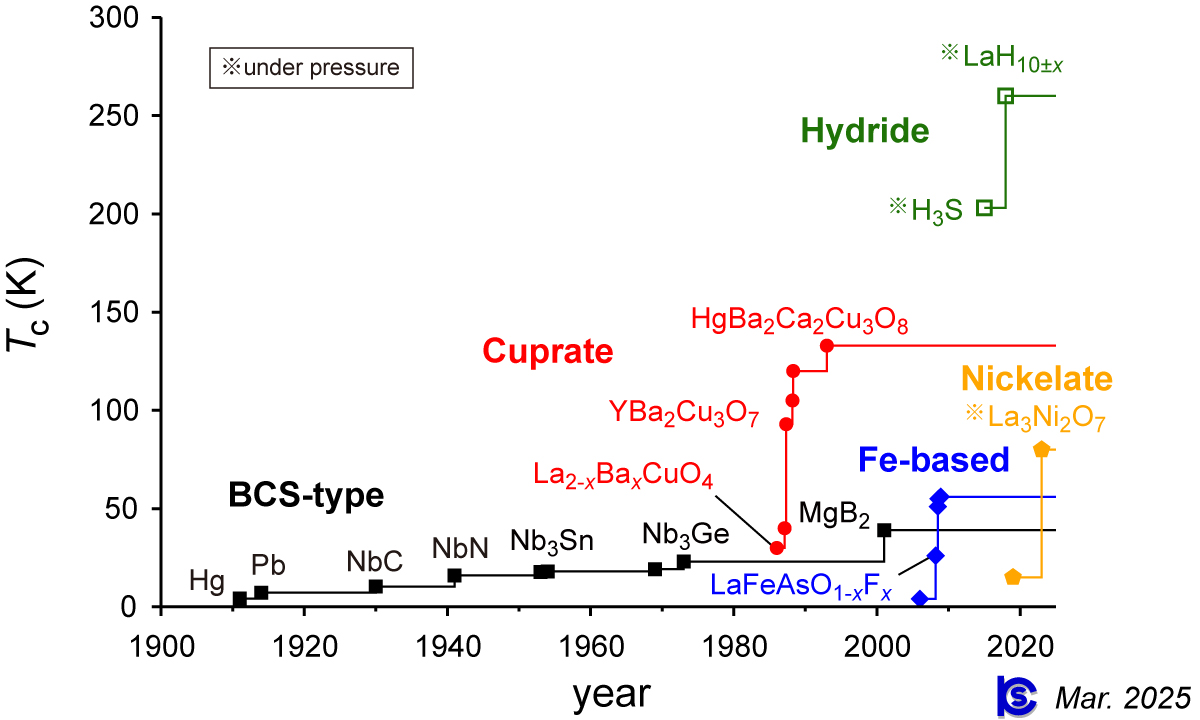
\includegraphics[width=0.9\textwidth]{tc-history_2025.jpg}
    \caption{超伝導転移温度の記録}
    \label{fig:tc-history}
\end{figure}
%東京大学 大学院総合文化研究科 広域科学専攻 相関基礎科学系 橘高研究室
%\url{https://park.itc.u-tokyo.ac.jp/kittaka/contents/others/tc-history/index.html}

Hartnollのレビュー!!!!!!!!!!!!!!!!!!!!!!

厳密にはマイスナー効果は起こらないが
マイスナー効果を引き起こすための本質的な物理
London方程式は導出されている

なぜ厳密には起こらないのか?

HHH論文自身が明確に述べている通り、このモデルでは電流が電磁場を生み出さないため、
厳密な意味でのマイスナー効果は存在しえません
マイスナー効果とは、超伝導体内部に生じた電流が、
外部磁場を打ち消すような逆向きの磁場を「自ら」作り出すことで磁場を排除する現象
電流が磁場を生み出せない設定である以上、この現象は起こり得ません 。

HHH論文の非常に重要な功績は、このモデルを用いて
ロンドン方程式 $J_i = -n_s A_i$ を導出したことです
ロンドン方程式は、ベクトルポテンシャル$A_i$ が存在するだけで(つまり磁場が存在するだけで)
電流 $J_i$ が流れることを示す、超伝導の根幹をなす関係式です 。
著者らは、このロンドン方程式が成立することを示した上で、
「もしこの理論を(後から)弱くゲージ化して、電流がマクスウェル方程式に従って磁場を生み出すようにすれば、
磁場は排除されるだろう」と論じています 。

つまり、HHH論文のモデルは、マイスナー効果という「現象」そのものは示しませんが
その現象を引き起こす原因である「ロンドン方程式」が、
このホログラフィックなセットアップから自然に導出されることを初めて示したのです。










新旧の違い!!!!!!!!!!!!!!!!!!!!!!!

従来模型 (HHH論文):

境界でのU(1)対称性はグローバル対称性
境界の電磁場(光子)が力学(ダイナミクス)を持たず外部から固定された**「外部ソース」**としてのみ存在

このモデルでは、外部からかけた電磁場に対して物質(超伝導体)がどのように応答し、
どんな電流$\langle J \rangle$ が流れるかを計算します。
しかし、その電流が電磁場自体にフィードバックを与える効果は、モデルの内部では考慮されません 。

新規模型 (Natsuume論文):
境界での電磁場を
ダイナミカルな場として扱います 。
これを実現するために、「半古典的なマクスウェル方程式 ($\nabla F = e^2 \langle J \rangle$)」
そのものを境界条件として課します 。
これにより、物質が生み出す電流 $\langle J \rangle$ が、電磁場 $F$ を変化させるという
バックリアクションがモデルに最初から組み込まれています。

従来模型が「固定された磁場に物質がどう応答するか」を見るのに対し、
新規模型は「磁場と物質が互いに影響を及ぼしあう、自己無撞着な状態」を直接解いている













\section{より現実的なモデルにするために}

上で作った模型は現実の超伝導の解析という目的からすると多くの問題があります.
\begin{itemize}
    \item Meissner効果が起こらない
    \item ラージNゲージ理論になっている
    \item AAA
\end{itemize}
ここでは
のMeissner効果が起こらないについて

作用にはMaxwell場が入っているじゃないかと思われるかもしれませんが,

Natsuume論文の新規模型は、HHH論文などで確立された従来模型の「外部ソース」という制限を取り払い、
電磁場のダイナミクスを直接組み込むことで、従来は間接的にしか示唆できなかったマイスナー効果を、
モデル内で直接的かつ解析的に示すことに成功した

\subsection{ホログラフィックMeissner効果}




\subsection{5次元模型}

ホログラフィック繰り込みの考えから境界に対数項$S_{\text{ct}}$が必要となる.
オンシェル超重力作用$S_{\text{sugra}}$の発散は、
バルク時空の境界(カットオフ$\rho = \epsilon$または$r^2 = \epsilon$)で評価されますが、その発散の構造は境界次元$d$に依存します。
• 奇数次元の場合: 発散項は$\epsilon$の逆べき乗($\frac{1}{\epsilon^k}$)の形のみで出現します。
• 偶数次元の場合: $\epsilon$の逆べき乗の項に加えて、対数発散項$\log \epsilon$が出現します


対数発散は、ホログラフィック繰り込みにおいて特殊な対処を必要とします。

作用を有限化するためには、この$\log$の発散も打ち消すように、
境界対項$S_{ct}$を含めなければなりません\cite{deHaro00}.






夏梅のレビュー!!!!!!!!!!!!!!!!!

超伝導らしきものを再現するための作用
s波ホログラフィック超伝導

理論モデル
4(5)次元時空(バルク)中のアインシュタイン・マクスウェル・スカラー理論
ホログラフィック超伝導体を記述する標準的なモデル
背景時空
バルクの時空は、ブラックホールが存在するSchwarzschild-AdS$_4$(5)時空
このブラックホールのホーキング温度が、境界の(2+1)(3+1)次元時空の温度に対応

\begin{equation}
    \begin{split}
        S_{\text{bulk}}
        &= \int \dd^4 x \sqrt{-g} \left( \mathcal{L}_g + \mathcal{L}_{\text{matter}} \right)\\
        \mathcal{L}_{g}
        &= R - 2 \Lambda\\
        \mathcal{L}_{\text{matter}}
        &= - \frac{1}{g^2} \left( \frac{1}{4} F^{MN} F_{MN} + |D_M \Psi|^2 + m^2 |\Psi|^2 \right)
    \end{split}
\end{equation}

ただし
\begin{equation}
    \begin{split}
        F_{MN} &= \partial_M A_N - \partial_N A_M,\\
        D_M &= \nabla_M - i A_M,\\
        \Lambda &= - \frac{3}{L^2}.
    \end{split}
\end{equation}

Maxwell場およびスカラー場が重力場と結合しない.
解析を簡単にするためにプローブ近似
$g \gg 1$ (or $q \to \infty$)
をとることで物質場から重力への影響・バックリアクションを無視できるようにする.

運動方程式は
どうこう

$A_u = 0$のゲージをとる
運動方程式は
どうこう

物質場の漸近的振る舞いは
\begin{equation}
    \begin{split}
        A_\mu &\sim \mathcal{A}_\mu+A_\mu^{(+)} u,\\
        \Psi &\sim \Psi^{(-)} u^{\Delta_{-}}+\Psi^{(+)} u^{\Delta_{+}},\\
        \Delta_{\pm} &\coloneq \frac{3}{2} \pm \nu, \quad \nu = \sqrt{\frac{9}{4}+m^2}.
    \end{split}
\end{equation}

\begin{equation}
    \begin{split}
        \ev{\mathcal{J}_\mu} &= \left.\frac{1}{g^2} F_{u \mu}\right|_{u=0} \\
        \ev{\mathcal{O}} &=\frac{1}{g^2} 2 \nu \Psi^{(+)}.
    \end{split}
\end{equation}

AdS/CFT辞書: バルクの場の境界近く($u \to 0$)での振る舞いが、境界の物理量に対応します。

バルクのベクトルポテンシャル
$A_\mu$の境界値$\mathcal{A}_\mu$が境界のベクトルポテンシャル
$A_\mu$の次のオーダーの項$A_\mu^{(+)}$が境界の電流$\ev{\mathcal{J}_\mu}$に対応する



バルクのスカラー場
$\Psi$の境界での主要項$\Psi^{(+)}$が超伝導の秩序パラメータ$\ev{\mathcal{O}}$に対応する


$\mathcal{A}_t = \mu$は化学ポテンシャルを
$A~{(+)}_t$は荷電密度$\ev{\rho}$を
同様に$\mathcal{A}_i$はベクトルポテンシャルを
$A^{(+)}_i$はカレント密度$\ev{\mathcal{J_i}}$を
$\Psi^{(+)}$はオーダーパラメータ$\ev{\mathcal{O}}$を
$\Psi^{(-)}$はオーダーパラメータの外場ソースを表す



Section III: Small Magnetic Field (小さい磁場をかけた場合)
ここがこの論文の最初の核心部分です。一定の超伝導状態に、弱い磁場をかけてみて、その応答を調べることでマイスナー効果を解析します。

A. Dirichlet Boundary Condition (通常の境界条件)
まず、従来の手法、つまり境界の電磁場
$\mathcal{A}_\mu$ を固定するディリクレ境界条件で計算するとどうなるかを見ています 。


計算: バルクのマクスウェル方程式 (3.2)  を解くと、境界での電流
$\ev{\tilde{\mathcal{J}}_y}$ は、境界のベクトルポテンシャル $\tilde{\mathcal{A}}_y$ を用いて
次のように書けることを導出します($q$ は運動量)。

\begin{equation}
    \begin{split}
        \ev{\tilde{\mathcal{J}}_y}& =\left.\partial_u \tilde{A}_y\right|_{u=0} \\
        & =\tilde{\mathcal{A}}_y\left(-q^2-2 \int_0^1 d u\left|\varphi_0\right|^2+\cdots\right)
    \end{split}
\end{equation}
電流は2つの部分からなる
超電流
$-2\int |\varphi_0|^2$ の項は、超伝導電子による電流ですこれはロンドン方程式に対応
束縛電流
$-q^2$の項は超伝導凝縮がない($\varphi_0=0$)通常の状態でも存在する電流
論文ではこれが物質の磁化による束縛電流として解釈できると指摘
境界のマクスウェル方程式(アンペールの法則)が存在しないため
(境界条件として電流が存在するだけで、Maxwell場はダイナミカルに存在はしない)
超電流が磁場を押し返すことができず、マイスナー効果は起こりません
磁場は超伝導体内部に自由に侵入できてしまいます

元の境界条件
$\mathcal{A}_\mu = \left. A_\mu \right|_{u = 0}$






新たな境界条件
非自明な解をとるために外場ソース$\mathcal{J}_{\text{ext}}^i$を加えてやる
\begin{equation}
    \partial_{j} \mathcal{F}^{ij}
    = e^{2} \left( \ev{\mathcal{J}^{i}} + \mathcal{J}_{\text{ext}}^i \right)
\end{equation}

\begin{equation}
    q^2 \tilde{\mathcal{A}}_y
    = \frac{e^2}{1 + e^2} \tilde{\mathcal{J}}^{\text{ext}}_y
    \coloneq \mu_m \tilde{\mathcal{J}}^{\text{ext}}_y
\end{equation}











\begin{equation}
    \begin{split}
            \mu_m
            &= \frac{e^2}{1 + e^2 / r_0}\\
            \chi_m
            &= - \frac{e^2 / r_0}{1 + e^2 / r_0}\\
            \lambda^2
            &= \frac{1 + e^2 / r_0}{2 e^2 I}\frac{1}{r_0}
    \end{split}
\end{equation}


















各種表式を代入してやり,Fourier変換などをいろいろして解く(方程式を出す)



結果の話

Meissner効果
\begin{equation}
    \mathcal{A}_{y}\propto e^{-x/\lambda}
\end{equation}
$\lambda$は磁場侵入長

境界での電流には、超伝導電子による
超電流の他に、物質の磁化に由来する束縛電流 (bound current) が存在する
束縛電流の効果により、物質の透磁率$\mu_m$ が真空の値からずれ,物性が変化

極端な第一種超伝導体にはなれない:

通常のギンツブルグ・ランダウ(GL)理論では、結合定数$e$を大きくすると
$e\rightarrow\infty$ で磁場侵入長がゼロ $\lambda \to 0$ となり、
磁場を完全に排除する極端な第一種超伝導体になります
しかし、このホログラフィックなモデルでは、束縛電流の効果により
$e\rightarrow\infty$ としても $\lambda$ が有限の値を保ち、極端な第一種にはなれないことが示されました

GLパラメータの導出(5次元バルクの場合):
特に解析的な解が得られる5次元バルクのモデルにおいて、磁場侵入長$\lambda$とコヒーレンス長 $\xi$ を具体的に計算し、
超伝導体の種類(第一種か第二種か)を決定するGLパラメータ $\kappa^2 = \lambda^2 / \xi^2$ を解析的に導出
超伝導体の性質が温度や結合定数にどう依存するかが明らかになりました


\bibliography{sohosai2025}
\bibliographystyle{junsrt}

\end{document}